\chapter{The Wavefunction}
  \section{Position representation }
  We start naturally from the postulates of quantum mechanics, having the state ket $ | \psi(t) \rangle $ ( in Schr\"{o}dinger's picture) that evolves in time by Schr\"{o}dinger's equation:
  \begin{equation}
  \hat{H} | \psi(t) \rangle = i \hbar \dfrac{\partial}{\partial t} | \psi(t) \rangle
  \end{equation}
  What we are interested in knowing for a free particle is its position, we therefore project the state ket into the position space , and get the \textbf{wavefunction}:
  \begin{equation}
  \psi (x,t) = \langle x | \psi (t) \rangle 
  \end{equation}
  The Hilbert space is therefore : $ \mathcal{H} \overset{\text{def}}{=} L ^2 (\; \; ] -\infty,+\infty[\; ;\; dx\; \; )$ \footnote{ This Hilbert space implies that the particle could be \textit{anywhere} in the universe until measured; \textbf{but the propability vanishes at infinity points} }The position operator is simply a multiplicative operator :
  \begin{equation}
  \hat{X} \psi (x,t) = x \psi(x,t) 
  \end{equation}
  It has a continuous spectrum of eigenvalues being the position(s) of the quantum particle in the 1-dimensional space. Generalisation to 3-D space is straightforward - see homework- . The task now is to find the momentum operator in the position representation, this can be done from investigating the canonical commutation relation $ [\hat{X}, \hat{p}_x]= i \hbar \hat{I}$, as following:
  \begin{align}
  [\hat{X}, \hat{p}_x] \psi(x,t)=& i \hbar \psi(x,t)  \nonumber \\
  x \hat{p}_x \psi(x,t) - \hat{p}_x ( x \psi (x,t)) =& i \hbar \psi (x,t) 
  \end{align}
  Rearranging the above equation :
  \begin{align}
  \hat{p}_x ( x \psi (x,t)) &= - i \hbar \psi (x,t)  + x \hat{p}_x \psi(x,t)\nonumber\\
  \Leftrightarrow \; \; \hat{p}_x ( x \psi (x,t)) &=\frac{\hbar}{i} \dfrac{\partial}{\partial x}\left( x \psi (x,t) \right) 
  \end{align}
  Hence we conclude that the momentum operator in the position representation is given by :
  \begin{equation}
  \boxed {\hat{p}_x \overset{\text{ def}}{=} \frac{\hbar}{i} \dfrac{\partial}{\partial x}}
  \end{equation}
  \section{Separation of variables in Schr\"{o}dinger's equation}
  Now, we attempt to quantise the free particle system. This is done first by defining the wavefunction and the Hilbert space. Now what is left is to quantise the Hamiltonian; recall that the Hamiltonian for the free particle is given by:
  \begin{equation}
  H (p)= \dfrac{p^2}{2m}
  \end{equation}
  The Hamiltonian operator that acts on the free-particle Hilbert space is $ \hat{H} = \dfrac{\hat{p}^2}{2m}$, since we have the position representation for the momentum operator $ \hat{p}$. We have the Hamiltonian operator:
  \begin{equation}
  \hat{H} \overset{\text{def}}{=}- \frac{\hbar ^2}{2 m} \dfrac{\partial ^2}{\partial x^2}
  \end{equation}
  Plunging it in the Schr\"{o}dinger's equation; to obtain:\marginpar{}
  \begin{equation}
  - \frac{\hbar ^2}{2 m} \dfrac{\partial ^2 \psi (x,t)}{\partial x^2}= i \hbar \dfrac{\partial \psi(x,t)}{\partial t }
  \label{SE}
  \end{equation}
 Observe the similarity between Schr\"{o}dinger's equation and the classical wave equation. However, we have derived this equation from an axiomatic approach. In order to solve \eqref{SE} we need to use a mathematical trick known as the\textbf{ separation of variables}. Assume that we can write the wavefunction as the product of two functions:
  \begin{equation}
  \psi(x,t) = \varphi (x) h(t)
  \end{equation}
  Substituting in \eqref{SE}, and rearranging, we obtain:
  \begin{equation}
  - \frac{\hbar ^2}{2 m }\; \frac{1}{\varphi(x)} \dfrac{d^2 \varphi{(x)}}{dx^2} = i \hbar \frac{1}{h(t)} \frac{d h(t)}{dt}
  \label{SE2}
  \end{equation}
  Each side of the equation \eqref{SE2} depends only on one variable, and since they equal each other. This implies :
  
  \begin{subequations}
  	\begin{equation}
  	- \frac{\hbar ^2}{2 m }\; \frac{1}{\varphi(x)} \dfrac{d^2 \varphi{(x)}}{dx^2} = \text{Const.} 
  	\end{equation}
  	\begin{equation}
  	i \hbar \frac{1}{h(t)} \frac{d h(t)}{dt}= \text{Const.}
  	\label{TDSE}
  	\end{equation}
  \end{subequations}
  Evidently, the 'constant' is indeed the eigen-energy of the particle $ E$. We start by solving the second equation \eqref{TDSE}, the solution yields, what-so-called the \textbf{stationary states} time evolution:
  \begin{equation}
  h(t) = e^{- i \omega t}. 
  \end{equation}
  with $ \omega = \frac{E}{\hbar}$. Observe this result can be obtained directly from the Heisenberg picture ( Show how !) All systems of which we can separate their time dependence in this way is called stationary states. They shall be the main focus in these notes. 
  \section{The free-particle solution}
  We now turn to the spacial part of Schr\"{o}dinger's equation
  \begin{equation}
  - \frac{\hbar ^2}{2 m }\; \dfrac{d^2 \varphi{(x)}}{dx^2} = E \varphi(x)
  \label{sch}
  \end{equation}
  This has a particular solution of the form
  \begin{equation}
  u(x) = C e^{i kx}
  \label{PW}
  \end{equation}
  With $ k^2 = \frac{ 2mE}{\hbar^2}$, having the dimension of inverse length; we recognise $ k$ being the wavenumber. The solution \eqref{PW} can be written in terms of the momentum - by the relation $ p = \hbar j$.-:
  \begin{equation}
  u(x) = C e^{\frac{i}{\hbar} p x}
  \label{PWp}
  \end{equation}
  This solution is known as the plane wave solution. It represents a wave propagating in the $ +x$ direction. This solution can be used to find $ \varphi(x)$ by the superposition principle; the 'constant' of integration is not constant in fact. Rather, it is a function of $ p$ . In order to see this, recall that the eigen-energy of the free particle $ E = \frac{p^2}{2m}=  \frac{(\hbar k)^2}{2m}$ putting this in \eqref{SE} we shall have a continuous spectrum of eigen-energies. Then use the spectral theorem we shall have therefore :
  \begin{equation}
  \varphi(x) = \frac{1}{\sqrt{2 \pi} \hbar} \int_{- \infty}^{+ \infty} \tilde{\varphi}(p) e^{\frac{i}{\hbar} p x} dp 
  \label{packet}
  \end{equation} 
  Which is simply the  Fourier transform of the momentum wavefunctions $ \tilde{\varphi}(p)  = \langle p | \varphi \rangle $ . We then identify the plane-wave solution as $ \langle x|p \rangle = e^{\frac{i}{\hbar} p x}$ . We can use the wavefunctions to calculate the probability of finding the particle as a given position $ x'$,  $ | \varphi(x')| ^2$ or momentum $ p'$ ,   $ | \tilde{\varphi}(p')| ^2$ . \\
  Since momentum cannot be determined with absolute certainty; it then takes a Gaussian wavefunction. Of which its Fourier transform is a Gaussian function itself. The figure \ref{timeevolution} is generated by a code we have made showing the time evolution of the wavefunction $ \psi (x,t)$, given an initial width for the momentum wavefunction Gaussian :
  \begin{figure}[h!]
  	\centering 
  	\label{timeevolution}
  	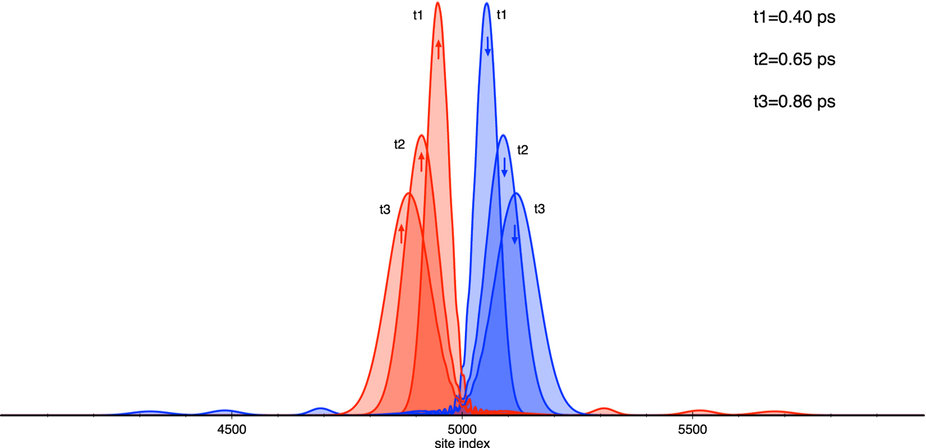
\includegraphics[width = 0.8 \textwidth]{./figures/packet.jpg}
  	\caption{Simulated time evolution of a Gaussian wavefunction for the free particle, observe the dispersion of the wave as time progresses }
  \end{figure}
  Observe how the wavefunction - indicating our certainty of the particle's position- gets wider and wider as time progresses. The equation \eqref{packet} indicates that the position wavefunction is composed of infinite number of momentum wavefunctions. The movement of the quantum particle is therefore expressed in terms of a \textbf{wavepacket} resulting from infinite number of waves interfering; we have run a computer code representing the wavepacket as seen in figure \ref{wavepacket} :
  \begin{figure}[h!]
  	\centering 
  	\label{wavepacket}
  	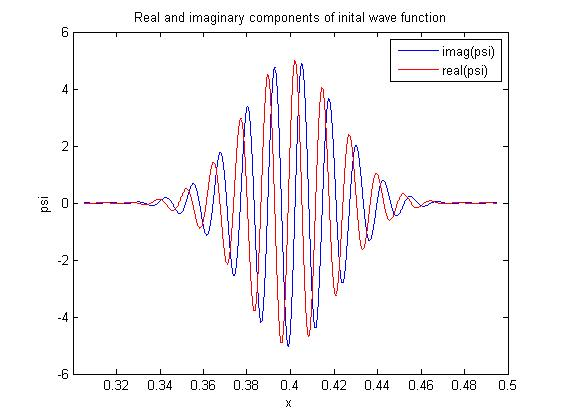
\includegraphics[width = 0.8 \textwidth]{./figures/wavefunction.jpg}
  	\caption{The wavepacket of the free quantum particle $ \psi(x,t)$ }
  \end{figure}
  \section{Probability flux and density }
  Since $| \psi (x,t)|^2 $ gives the probability of finding the particle at any point in space, at a given time. It defines a positive real-valued function of space. It is known as the p\textbf{probability density function}:
  \begin{equation}
  \rho (x,t) = \psi^* (x,t) \psi (x,t)
  \end{equation}
  We also define the probability current density 
  \begin{equation}
  j(x,t) = \frac{\hbar}{2mi}\left( -\dfrac{\partial \psi^* (x,t)}{\partial x} \psi (x,t) + \psi^* (x,t)\dfrac{\partial \psi (x,t)}{\partial x} \right) 
  \end{equation}
  let's now look at $ \dfrac{\partial j (x,t)}{\partial   x}$ :
  \begin{align}
  \dfrac{\partial j (x,t)}{\partial x} =& \dfrac{d}{dx}\left[ \frac{\hbar}{2mi}\left( -\dfrac{\partial \psi^* (x,t)}{\partial x} \psi (x,t) + \psi^* (x,t)\dfrac{\partial \psi (x,t)}{\partial x} \right) \right] \nonumber \\
  =& \frac{\hbar}{2mi}\left( -\dfrac{\partial^2 \psi^* (x,t)}{\partial x^2} \psi (x,t) - \dfrac{\partial \psi^* (x,t)}{\partial x} \dfrac{\partial \psi (x,t) }{\partial x } +\right.\nonumber \\ 
  &\qquad\left. {} \psi^* (x,t)\dfrac{\partial ^2 \psi (x,t)}{\partial x^2} +  \dfrac{\partial \psi^* (x,t)}{\partial x} \dfrac{\partial \psi (x,t) }{\partial x }\right) \nonumber \\
  =& \frac{\hbar}{2mi}\left( -\dfrac{\partial^2 \psi^* (x,t)}{\partial x^2} \psi (x,t) + \psi^* (x,t)\dfrac{\partial^2 \psi (x,t)}{\partial x^2} \right) 
  \end{align}
  We can also calculate $ \dot{\rho}(x,t)$:
  \begin{align}
  \dot{\rho}(x,t) =& \dfrac{\partial }{\partial t }\left( \psi^* (x,t) \psi (x,t)\right) \nonumber \\
  =&  \dfrac{\partial \psi^* (x,t) }{\partial t } \psi (x,t) + \psi^* (x,t) \dfrac{\partial \psi (x,t) }{\partial t }
  \end{align}
  But from Schr\"{o}dinger's equation, we have $ \dfrac{\partial \psi (x,t) }{\partial t } = \frac{-\hbar}{2m i }\left(  \dfrac{\partial^2 \psi (x,t)}{\partial x^2}\right) $. Hence we incur:
  \begin{align}
  \dot{\rho}(x,t) =& \frac{\hbar}{2mi}\left( \dfrac{\partial^2 \psi^* (x,t)}{\partial x^2} \psi (x,t) - \psi^* (x,t)\dfrac{\partial^2 \psi (x,t)}{\partial x^2} \right)
  \end{align}
  \begin{equation}
  \Leftrightarrow \dfrac{\partial j (x,t)}{\partial x} + \dot{\rho}(x,t)=0
  \end{equation}
  
  This is the continuity equation in quantum mechanics , implying probability is conserved .
  \section{ The Born conditions}
  Max Born’s best known contribution to quantum mechanics was his proposal that the wave function, or rather its square modulus, should be interpreted as the probability density for finding the system in a given state at a given time. However, he also proposed four conditions on the wave function which are used in finding many solutions of the Schr\"{o}dinger equation. As always, it’s useful to take another look at the Schr\"{o}dinger equation (in one dimension \eqref{sch}) so we can see how  Born's conditions fit in.\\
  Born’s conditions to be imposed on the wave function $\psi(x,t)$ are:
  \begin{enumerate}
  	\item he wave function must be single valued. This means that for any given values of$x$ and $\psi(x,t)$  must have a unique value. This is a way of guaranteeing that there is only a single value for the probability of the system being in a given state. 
  	\item The wave function must be square-integrable. In other words, the integral of $ | \psi| ^2$ over all space must be finite. This is another way of saying that it must be possible to use $ | \psi| ^2$ as a probability density, since any probability density must integrate over all space to give a value of 1, which is clearly not possible if the integral of $ | \psi| ^2$ is infinite. One consequence of this proposal is that $ \psi$ must tend to 0 for infinite distances. 
  	\item The wave function must be continuous everywhere. That is, there are no sudden jumps in the probability density when moving through space. If a function has a discontinuity such as a sharp step upwards or downwards, this can be seen as a limiting case of a very rapid change in the function. Such a rapid change would mean that the derivative of the function was very large (either a very large positive or negative number). In the limit of a step function, this would imply an infinite derivative. Since the momentum of the system is found using the momentum operator, which is a first order derivative, this would imply an infinite momentum, which is not possible in a physically realistic system. Such an infinite derivative would also violate condition 4. 
  	\item All first-order derivatives of the wave function must be continuous. Following the same reasoning as in condition 3, a discontinuous first derivative would imply an infinite second derivative, and since the energy of the system is found using the second derivative, a discontinuous first derivative would imply an infinite energy, which again is not physically realistic. 
  \end{enumerate}
\section{Problems}
  \begin{enumerate}
  	\item Calculate $\langle p\rangle$  and  $\langle E\rangle$ for the free particle 
  	\item We define the 'group velocity' $ v_g$ for a wavepacket as:
  	\[
  	v_g = \frac{d \omega}{dk}
  	\]
  	Show that this equals the 'classical velocity' for the particle.
  	\item We define the `phase velocity' $ v_p$ as:
  	\[
  	v_p =\frac{ \omega}{  k}
  	\]
  	Show it equals half of the classical velocity.
  	\item If the momentum wavefunction $ \tilde{\varphi}(p) \rightarrow \delta(p-p_0)$. Write down $\psi(x,t)$ explicitly. What do you observe ?
  	\item Show that in Heisenberg picture, we arrive to the same stationary states solution $ e^{-i \frac{E t}{\hbar}}$
  	\item Show that the free particles could have both $ k>0$ and $ k<0$, i.e $ e^ {-ikx}$ is also a solution to the free particle. What does that mean physically ?
  	\item Write Schr\"{o}dinger's equation for the free particle in 3 dimensions. 
  \end{enumerate}
  \nocite{*} 